\documentclass{article}

\usepackage{amsmath}
\usepackage{amsfonts}
\usepackage{listings}
\usepackage{algpseudocode}
\usepackage{mathtools}
\usepackage{qtree}
\DeclarePairedDelimiter{\ceil}{\lceil}{\rceil}
\DeclarePairedDelimiter{\floor}{\lfloor}{\rfloor}

\title{Proposal}

\author{Anton Pozharskiy}




\begin{document}
\begin{titlepage}
  \begin{center}
    \vspace*{1cm}
    
    \Huge
    \textbf{Independent Bi-ocular Active VIO}
    
    \vspace{0.5cm}
    \LARGE
    Project Proposal
    
    \vspace{1.5cm}
    \Large
    \textbf{Anton Pozharskiy}
    
    \vfill

    \vspace{0.8cm}
    
    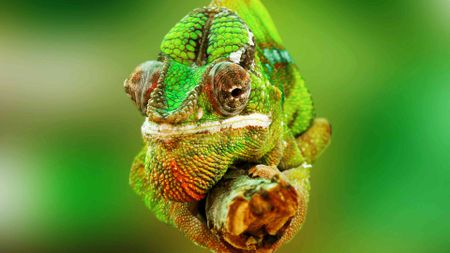
\includegraphics[width=0.5\textwidth]{Chmln}
    
    \Large
    Computer Science\\
    University of Maryland\\
    United States\\
    \today
    \end{center}
\end{titlepage}

\newpage

\section{Goals} %This is how I denoted problems and subparts of problems
This projects has several goals, to be completed in the following order
\begin{enumerate}
\item Build a test platform with two rotational 2-dof mounts, high-fov cameras, and IMUs.
\item Develop a tightly integrated VIO on each eye.
\item Develop a loosely integrated stereo VIO
\item Develop a Loop closure system to act on both eyes.
\item Develop a huristic decision making system to recalibrate scale between the two cameras.
\item Develop a gaze control system to improve VIO/SLAM performance 
\end{enumerate}
This is all in an attempt to allow for what is essentially a two loosely connected monocular SLAM system to
combat scale drift by being able to actively convert to a stereo system.

This project would aim to develop the logic for actively tracking and exploring feature rich areas. It would also
develop a heuristic method to readjust the scale factor by taking advantage of stereo images across the two
cameras. 
\section{Motivation}
Often natural systems are an inspiration for engineers. In this case the chameleons ability to independently
operate its two eyes in order to traverse trees and search for interesting targets, and have effective depth
preception.

It is a well documented feature of VSLAM that the larger the field of view the better quality the tracking tends
to be. Generally, cameras with high fields of vision come with downsides, primarily in the form of high levels of
distortion. In general this is solved with expensive arrays of cameras or mirrors. This approach is an attempt to
take advantage of the already explored avenues of activeSLAM, a technique that uses information metrics inherent in
SLAM systems to plan exploration and paths through an environment. That will be combined with the active tracking
of feature landmarks using an image salience technique in order for the system to automatically attempt to improve
its tracking performance. 

\section{State of the Art}
\subsection{Active Gaze Control}
There exist several approaches to active gaze control that have been explored. They are primarily used to
identify where in an image the algorithm should search for feature matches under loop closure. This approach is
used in [1] which Newman and Ho use it to improve loop closure detection. It is also used in the field of
``active SLAM'' where it is used to guide the camera in which direction to go in order to maximize feature overlap
[2]. As far as I can tell there is not a lot of research into active gaze control for stereo systems.

\subsection{Visual Inertial odometry}
There is also no state of the art for independent pairs of cameras. However, stereo visual odometry is a well
known technique as is monocular visual odometry. As for visual-inertial odometry there are several known aproaches.
They broadly fall into two seperate categories: Loose coupling and tight coupling. Loose coupling often involves
cascades of kalman filters in order to combine IMU readings with the visual odometry readings. Tightly coupled
approaches on the other hand pair imu measurements with camera frames in order to gain an advantage from getting
estimated ego-motion at the time of the frame capture. Both of these have their pros and cons, depending on hardware
type of motion etc. As stated before there is no research on how to link two independent cameras together with
a tight coupling, however many kalman filter based approaches have been used to combine multiple noisy pose
estimate in the past. 

\section{Tentative Plan}
As stated above there are several major parts to this project:

\begin{itemize}
\item Physical hardware:
  \begin{itemize}
  \item Cameras
  \item IMU's
  \item Gimbals
  \end{itemize}
\item Independent monocular VIO
\item Loop closure system
\item Scale realignment system.
\item Gaze control system
\end{itemize}

The current timeline is to have the physical system done by the end of spring break. After that in the next 3
weeks the independent VIO and loop closure system should be completed. In the final 4 weeks of the semester the
scale realignment heuristic and gaze control system should be implemented.

\end{document}

